\section{Sensor Considerations}
\label{sec:sensors}
At the time of writing, the Android Platform provides a large number of sensors\autocite{Android:Sensors}: 
\begin{itemize}
\item accelerometer including gravity
\item ambient temperature
\item accelerometer excluding gravity
\item current rotation of the phone
\item ambient light
\item ambient magnetic field
\item ambient air pressure
\item proximity to screen
\item ambient humidity
\end{itemize}
For detecting a users activity accelerometer and rotational sensors are obviously the most useful ones. The first idea pursued was to use a combination of rotational sensors as well as acceleration excluding gravity. After taking some measurements this approach was abandoned, because rotation is provided as number which will flip from its maximum value to its minimum at the end of its positive range. As depicted in \fref{myfig:rotation_sensor}, this would make feature extraction much more complicated.
\begin{figure}[htpb]
\centering
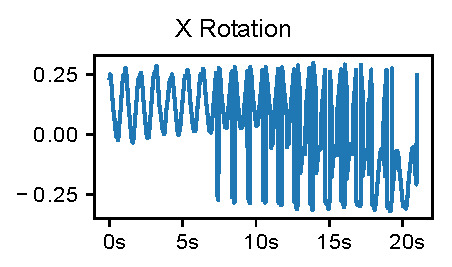
\includegraphics[width=\linewidth]{rotation_example.eps}
\caption{Examplary rotational sensor output recorded while walking.}
\label{myfig:rotation_sensor}
\end{figure}
Using the acceleration sensor without gravity is also a bad idea as this leads to an information loss. If the user has his phone in his pocket while sitting, gravity can be observed on the Z axis. In contrast it will be on the X axis, while he is standing.

This leads to the conclusion, that just using the acceleration sensor which includes gravity will lead to features which are easier to handle.

\section{Feature Selection and Windowing}
\label{sec:features}
The next task of this laboratory was to record measurements using the phone, transfer this measurements to a computer and define features which can later on be used in a \gls{knn} algorithm. To achieve this every class of activity was recorded four times. Three of these recordings were used for training and one to test classification using different features and ways of calculating them. In a first try the following features were calculated per test file:
\begin{itemize}
\item minimum of x acceleration
\item minimum of y acceleration
\item minimum of z acceleration
\item maximum of x acceleration
\item maximum of y acceleration
\item maximum of z acceleration
\item mean of x acceleration
\item mean of y acceleration
\item mean of z acceleration
\item standard deviation of x acceleration
\item standard deviation of y acceleration
\item standard deviation of z acceleration
\end{itemize}
This sums up to feature vectors whith a size of 12. For the \gls{knn} algorithm this means that three test files times six classes lead to a total of 18 samples. For the easier to detect classes like sitting and standing, this is already enough to work reliably. Classes which are harder to separate need a windowing approach which can be seen by comparing \fref{myfig:jogging_unwindowed} to \fref{myfig:jogging_windowed}.
\begin{figure}[htpb]
\centering
\includegraphics[width=\linewidth]{jogging_unwindowed.eps}
\caption{Classification with features generated without windowing.}
\label{myfig:jogging_unwindowed}
\end{figure}
\begin{figure}[htpb]
\centering
\includegraphics[width=\linewidth]{jogging_windowed.eps}
\caption{Classification with features generated with windowing.}
\label{myfig:jogging_windowed}
\end{figure}
Windowing was implemented by calculating one feature every \SI{1.2}{\second} over all files. To avoid the bias introduced by longer recordings leading to more features, the minimum amout available in all classes was chosen as a limit. The remaining feature vectors were discarded.

\section{Evaluating the KNN algorithm}
\label{sec:resultsKNN}
In the end of the first part of the laboratory, the \gls{knn} algorithm had to be implemented on the smartphone making use of the features precalculated on the computer. A video was recorded to demonstrate that the application is working. The recording was produced making use of the application \texttt{OBS-Studio}\autocite{obsproject:website}, as it is capable of mixing multiple streams. In detail, the screen of the smartphone as well as a camera stream of the recording device were used as sources.

\fref{myfig:knn_screenshot} shows one frame of the video. This frame shows the probabilities calculated by the \gls{knn} algorithm on the smartphone over time while the author of this report is jogging.
\begin{figure}[htpb]
\centering
\includegraphics[width=\linewidth]{knn_screenshot}
\caption{One frame of the proof video demonstrating the \gls{knn} algorithm in action. The graph at the bottom depicts the probability of jogging.}
\label{myfig:knn_screenshot}
\end{figure}

\section{Developing a Base Model}
\label{sec:baseModel}
The course organization introduced the students of this laboratory to machine learning approaches by showing them how to train a model using the publicly available WISDM dataset\autocite{wisdm:dataset}. Performance of the provided example code is depicted for comparison in \fref{myfig:PlainGithub}.
\begin{figure}[htpb]
\centering
\includegraphics[width=\linewidth]{PlainGithub}
\caption{Performance of the base model example code provided by the course organziation.}
\label{myfig:PlainGithub}
\end{figure}
From this starting point a lot of optimizations were tried.

The first idea was to normalize the raw acceleration data in a different way than in the example code, as better normalized input data leads to faster convergence of machine learning models\autocite{Medium:Normalization}. The results shown in \fref{myfig:StdScaler} were generated using the \texttt{StandardScaler} module of \texttt{scikit-learn}\autocite{scikit:learn}.
\begin{figure}[htpb]
\centering
\includegraphics[width=\linewidth]{StdScaler}
\caption{Performance of the base model with better normalized input data using \texttt{StandardScaler} of \texttt{scikit-learn}.}
\label{myfig:StdScaler}
\end{figure}
Unfortunately the validation accuracy using this method performed slightly worse than the one of the given solution and the validation loss also increased.

The second idea was to split the training data by activities. The code given by the course organization just windows over all training data and assigns it with the label of the majority of samples. As depicted in \fref{myfig:SplitActivity}, implementing this change made it impossible for the network to converge.
\begin{figure}[htpb]
\centering
\includegraphics[width=\linewidth]{SplitActivity}
\caption{Performance of the base model with input data split by activities before windowing and labelling.}
\label{myfig:SplitActivity}
\end{figure}

The third approach was to change the network structure from just a combination of dense layers to:
\begin{enumerate}
\item convolutional layer with a height of 64
\item dropout layer with \SI{20}{\percent}
\item convolutional layer with a height of 32
\item dropout layer with \SI{20}{\percent}
\item convolutional layer with a height of 6
\item global average pooling layer
\item dense layer with softmax activation
\end{enumerate}
Note that the last convolutional layer results in a data cube with the 6 output classes as height. The global average pooling layer makes this convolutional layer learn the required pattern for identifying these classes. This approach was inspired by Martin Görner\autocite{Google:withoutPHD}. It results in much less computational effort than finishing convolutional layers with one or more dense layers. The performance of this model during training is depicted in \fref{myfig:DidiConvFinal}.
\begin{figure}[htpb]
\centering
\includegraphics[width=\linewidth]{DidiConvFinal}
\caption{Performance of the base model with convolutional layers.}
\label{myfig:DidiConvFinal}
\end{figure}

In the end the improved base model's performance was measured using test data which was not shown to it during training or validation. The performance of the authors final model on this test data is depicted in \fref{myfig:DidiConvFinalConfusion} and can be compared to the model provided by the course organization in \fref{myfig:GithubConfusion}.
\begin{figure}[htpb]
\centering
\includegraphics[width=\linewidth]{GithubConfusion}
\caption{Confusion matrix showing the performance of the model provided by the course organization.}
\label{myfig:GithubConfusion}
\end{figure}
\begin{figure}[htpb]
\centering
\includegraphics[width=\linewidth]{DidiConvFinalConfusion}
\caption{Confusion matrix showing the performance of the model by the author.}
\label{myfig:DidiConvFinalConfusion}
\end{figure}
Accuracy and loss values are compared in \fref{tab:accLoss}.
\begin{table}
\centering
\begin{tabular}[htpb]{rcc}
                    & Accuracy & Loss \\
Course Organization & 0.72 & 1.13 \\
Author              & 0.77 & 0.57 \\
\end{tabular}
\caption{Performance of the authors model compared to the model given by the course organization.}
\label{tab:accLoss}
\end{table}

%\FloatBarrier
\section{Creating the Head Model}
\label{sec:headModel}
For transfer learning a pre-trained base model is cut at a certain layer and new untrained layers are appended to it. These layers are trained directly on the target device. The code to do so was initially developed by Aaqib Saeed\autocite{saeed:transferLearning} as an example which is able to identify two separate classes. It was extended to the six classes described in \fref{sec:intro} and adapted to the base model developed in \fref{sec:baseModel}.

\section{Android Implementation}
\label{sec:android}
Most of the code for implementing transfer learning and running \texttt{TensorFlow} models on an android device was already developed by Aaqib Saeed\autocite{saeed:transferLearning} and the \texttt{TensorfFlow Lite} framework. The \gls{gui} was implemented from scratch and plots the prediction results of the \gls{knn} algorithm, the base model and the transfer learning model over time.
A settings frame which is shown in \fref{myfig:settings} of the app makes it possible to tell it the current position of the smartphone on the users body.
\begin{figure}[htpb]
\centering
\includegraphics[width=\linewidth]{settingsFrame}
\caption{Screenshot of the settings frame of the android application.}
\label{myfig:settings}
\end{figure}

\section{Evaluating Machine Learning approaches}
\label{sec:resultsML}
The final goal of this laboratory was to compare classification results of the \gls{knn} algorithm with the base model and the transfer learning model. This was again done using a video recording as described in \fref{sec:resultsKNN}.

\fref{myfig:all_screenshot} shows one frame of this recording in which the author of this report is standing. \gls{knn} as well as the transfer learning model would correctly classify standing, as the smartphone is lieing in an angle similar to being in the pocket where the \gls{knn} measurements were taken. Unfortunately the base model thinks the user is going upstairs.
\begin{figure}[htpb]
\centering
\includegraphics[width=\linewidth]{all_screenshot}
\caption{One frame of the proof video demonstrating the comparison of all implemented algorithms.}
\label{myfig:all_screenshot}
\end{figure}

\fref{myfig:sitting} shows a screenshot which was taken while the user was sitting with the phone in its pocket. This situation also displays, that \gls{knn} and the transfer learning model trained to this location of the phone are working. In contrast \fref{myfig:knn_wrong_screenshot} shows a screenshot which was taken while the user is walking and has the phone attached to its hand like in \fref{myfig:all_screenshot}. In this situation the \gls{knn} algorithm performs worse, because it was trained with the phone in the pocket. The transfer learning model was trained on device with the phone attached to the users hand. This is why it is able to correctly classify walking in this situation.
\begin{figure}[htpb]
\centering
\includegraphics[width=\linewidth]{sitting}
\caption{Screenshot of the application taken while the user was sitting with the phone in its pocket.}
\label{myfig:sitting}
\end{figure}
\begin{figure}[htpb]
\centering
\includegraphics[width=\linewidth]{knn_wrong_screenshot}
\caption{Screenshot of the application taken while the user was walking with the phone attached to its hand.}
\label{myfig:knn_wrong_screenshot}
\end{figure}

To have a quantitative estimation of the apps performance, a logging functionality was implemented in the end. This made it possible to record classification results of all three methods into a file. One file per class and smartphone position was recorded and later on evaluated on a PC. This led to the results depicted in \fref{tab:classPerf}.
\begin{table}
\centering
\begin{tabular}[htpb]{rSSS}
                             & {KNN} & {TL} & {BM} \\
downstairs, phone on hand & 0.0 & 65.5 & 0.0 \\
jogging, phone on hand & 0.0 & 34.6 & 88.8 \\
sitting, phone on hand & 0.0 & 0.0 & 0.0 \\
standing, phone on hand & 100.0 & 62.4 & 0.0 \\
upstairs, phone on hand & 0.0 & 39.2 & 0.0 \\
walking, phone on hand & 0.0 & 28.5 & 0.0 \\
downstairs, phone in pocket & 34.7 & 0.0 & 0.0 \\
jogging, phone in pocket & 12.0 & 41.1 & 94.1 \\
sitting, phone in pocket & 100.0 & 100.0 & 0.0 \\
standing, phone in pocket & 100.0 & 0.0 & 0.0 \\
upstairs, phone in pocket & 0.0 & 0.0 & 0.0 \\
walking, phone in pocket & 88.0 & 100.0 & 0.0 \\
\end{tabular}
\caption{Classification performance of all three algorithms in percent.}
\label{tab:classPerf}
\end{table}